\chapter{Algorithmen}

TODO

\section{Globale vs. lokale Pfadplanung }

TODO

\begin{figure} %Von Website
	\centering
	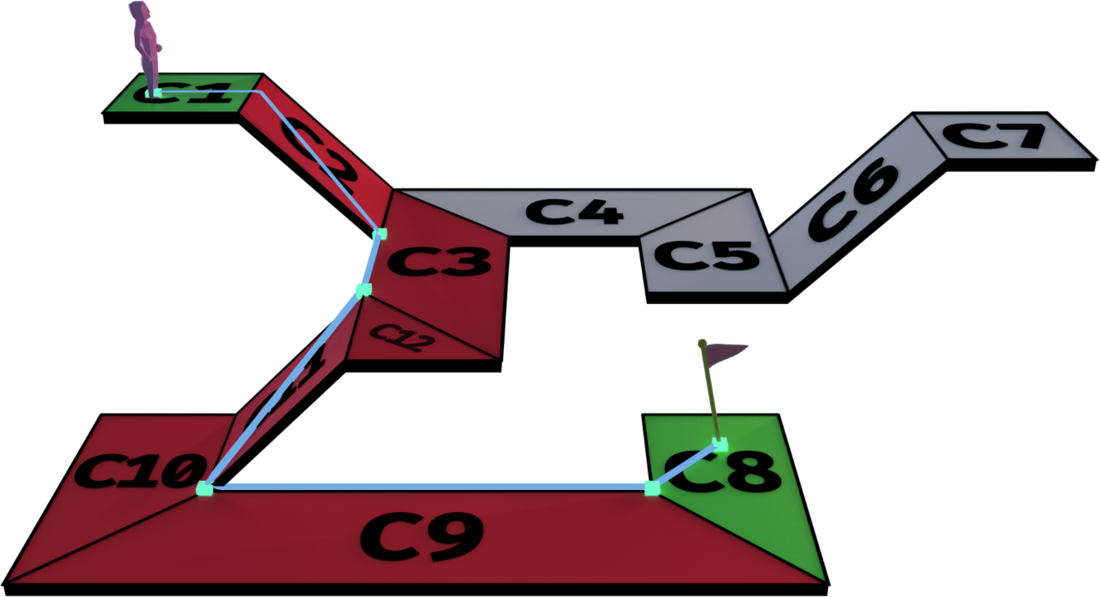
\includegraphics[width=\textwidth]{images/mesh_with_path.png}
	\caption{Von \cite{Mesh:18}: Navigation Mesh mit ein Pfad von Startpunkt C1 bis Endpunkt C2}
	\label{sec1a}
\end{figure}



\section{Sampling Algorithmen}
TODO



\section{Heuristiken}
TODO


\section{Pfadoptimierung}
TODO


\subsection{Umgebungswahrnehmung}
TODO


\subsection{Abh"angigkeit von dem Einsatzgebiet} 
TODO

\section{Funktionsweise popul"arer Algorithmen}
TODO

\subsection{A*-Algorithmus}
TODO

\subsection{IDA*-Algorithmus}
TODO

\subsection{RRT-Algorithmus}
TODO

\subsection{Weitere}
TODO
